% !TEX root = Hauptdatei.tex
\section{HMI Frameworks}
\label{hauptabschnitt_4}

Im Jahr 2017 wurden bereits diverse HMI Frameworks seitens Bosch evaluiert. An verschiedene Anbieter von \ac{HMI}-Frameworks wurde eine Anforderungsliste geschickt. Die erfolgversprechendsten Anbieter wurden eingeladen um verschiedene Use Cases in ihrem Framework umzusetzen. Das Ergebnis der Evaluation war, dass CGI Studio die Anforderungen am Besten abdeckt.\\

In diesem Kapitel werden Storyboard und Qt erneut evaluiert. Qt wurde ausgewählt weil es bei der Evaluation 2017 gut abgeschnitten hat. Hauptkritikpunkt war die fehlende 3D-Unterstützung. Storyboard wurde als Gegenpart zu Qt ausgewählt. Storyboard versucht, im Gegensatz zu Qt, mit wenigen einfachen Funktionen den größtmöglichen Nutzen zu bieten. \\ 

\subsection{CGI Studio}
\label{cgi}
Das Tool CGI Studio wird aktuell von Bosch für die \ac{HMI}-Entwicklung eingesetzt. Aufgrund der langjährigen Nutzung sind viele Entwickler mit der Nutzung von CGI Studio vertraut. Im Rahmen dieser Arbeit gab es jedoch einige Schwierigkeiten CGI Studio zu testen. Der Scene Composer, in dem das HMI erstellt wird, lädt beim Start eine DLL-Datei. In dieser DLL-Datei, sind die Widgets und Controls hinterlegt. Das Verhalten und die Funktionen der Widgets und Controls müssen vorher in C++ programmiert werden. Anschließend wird eine DLL-Datei daraus erzeugt. Das ermöglicht für jedes Projekt eigene Widgets zu programmieren.\\

Diese Vorgehensweise birgt allerdings auch Probleme. Das Wissen zu den verschiedenen Widgets und Controls liegt sehr konzentriert bei den Projektbeteiligten. Zusätzlich gibt es für jedes Projekt eine eigene DLL-Datei, dadurch ist es sehr unübersichtlich, welche DLL-Dateien, welche Widgets beinhalten. Auch ob die Widgets noch aktuell sind, ist nicht ersichtlich.\\

Daher kam es vor allem zu dem Problem, dass der Scene Composer des öfteren abgestürzt ist. Das Problem war eine schlechte Fehlerbehandlung innerhalb eines Widgets. Es stellte sich im Nachhinein heraus, dass dieses Widget veraltet ist. Deshalb liegt der Fokus auf die zwei Mitbewerber Storyboard und Qt, welche in den folgenden Kapiteln beschrieben werden.\\ 


\subsection{Storyboard}
Storyboard wird von der Firma Crank Software Inc. entwickelt, die in Kanada ansässig ist. Storyboard basiert auf der Eclipse Entwicklungsumgebung.
\glqq Eclipse [...] ist ein quelloffenes Programmierwerkzeug zur Entwicklung von Software verschiedener Art. Ursprünglich wurde Eclipse als integrierte Entwicklungsumgebung (IDE) für die Programmiersprache Java genutzt, aber mittlerweile wird es wegen seiner Erweiterbarkeit auch für viele andere Entwicklungsaufgaben eingesetzt. Für Eclipse gibt es eine Vielzahl sowohl quelloffener als auch kommerzieller Erweiterungen. \grqq \cite{wiki_storyboard}

%\begin{figure}[htb]
%	\centering
%	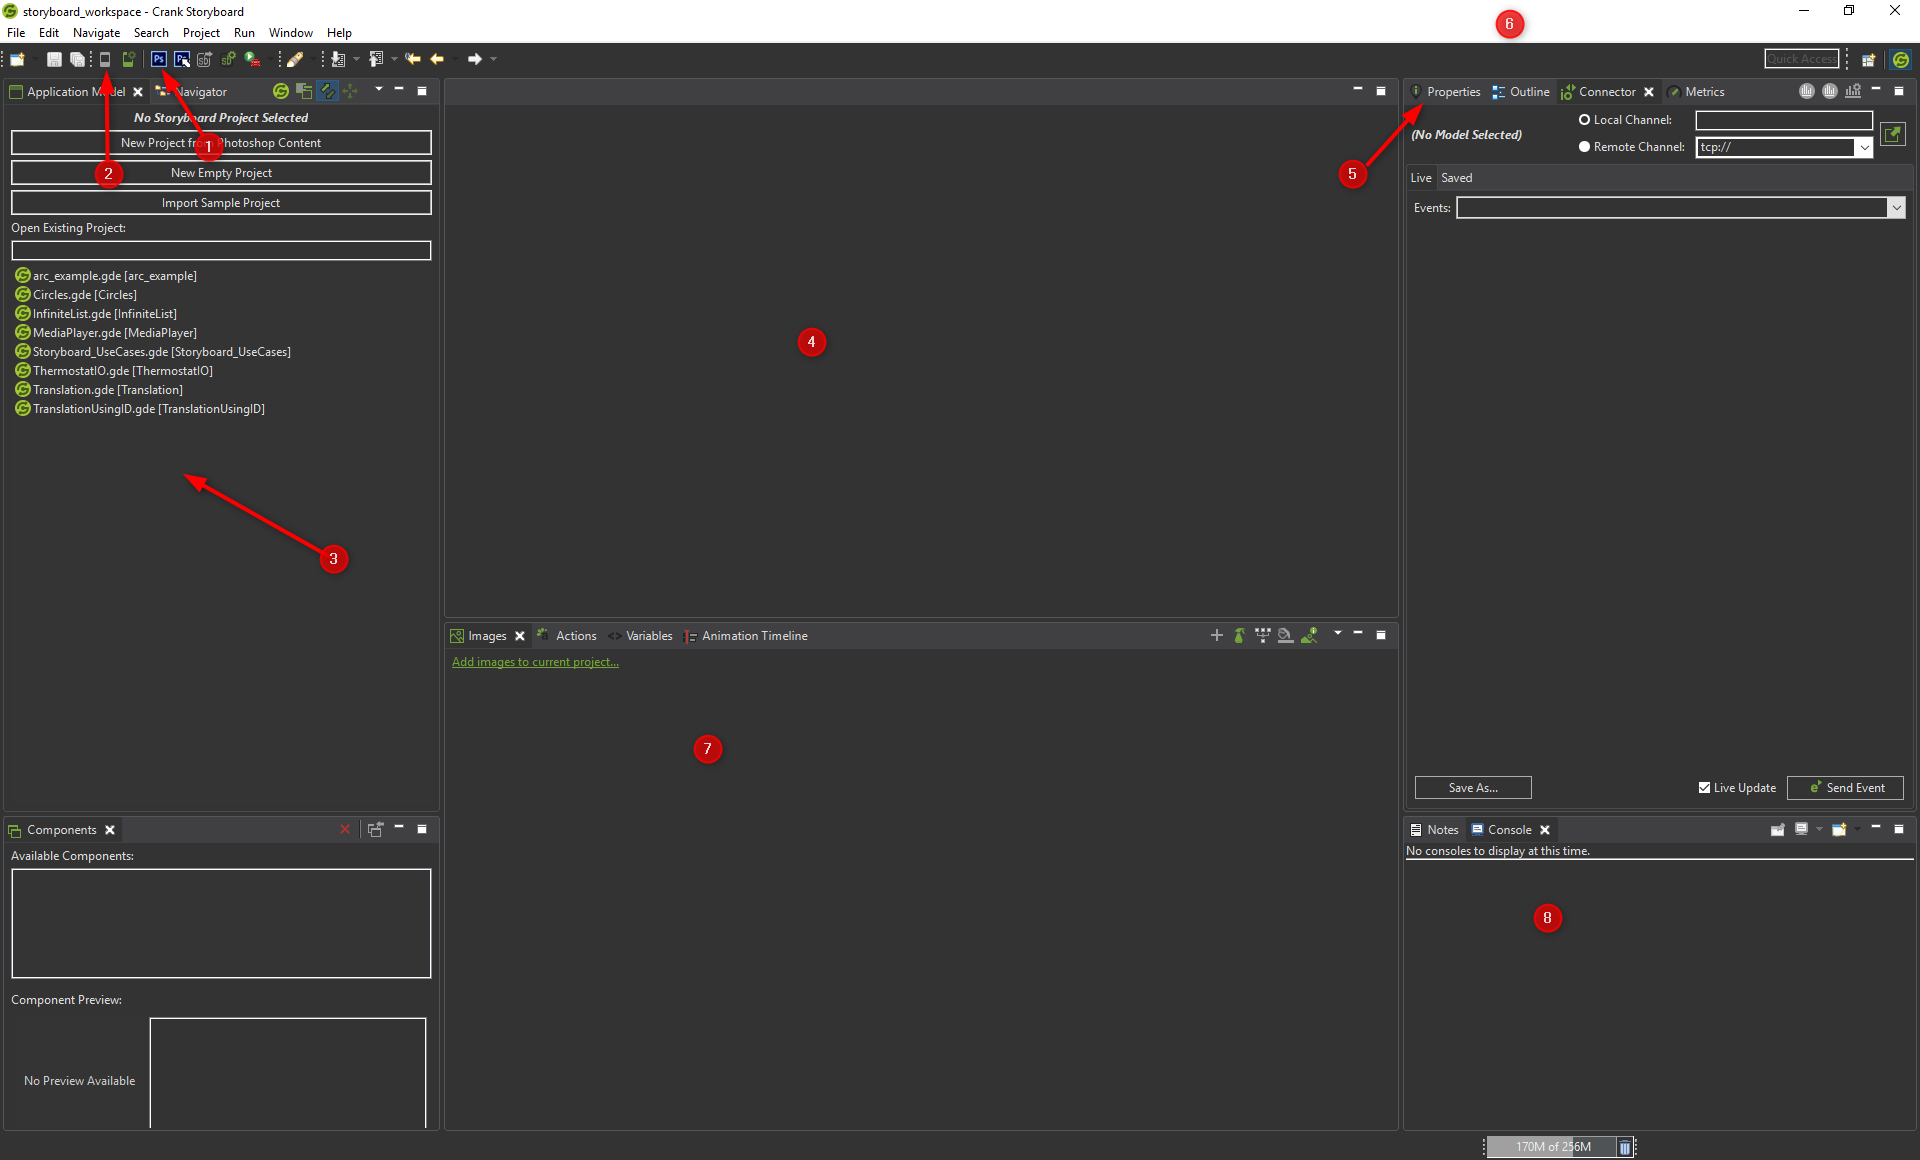
\includegraphics[width=\textwidth]{img/3_entwicklung_neues_kontept/2020-06-15_10h33_25}
%	\caption[Storyboard Start]{Storyboard Programm direkt nach dem Öffnen. 1: Photoshop-Import, 2: Simulation des Programms, 3: Auswahl der Bestehenden Projekte, 4: Editor, 5: Eigenschaften-Fenster, 6: Connector, 7: Bilder, Variablen, Actions, Timeline, 8: Konsolenausgabe}
%	\label{fig:storyboard_start}
%\end{figure}

%In Abbildung \ref{fig:storyboard_start} ist die grundsätzliche Aufmachung von Storyboard zu sehen. Von diesem Screen aus, können neue Projekte gestartet werden oder bestehende Projekte geöffnet werden.\\

%Das obere horizontale Menüband bietet die selben Funktionen wie in vielen anderen Programmen auch, es lassen sich Projekte und Dateien öffnen, neue Projekte und Dateien anlegen und diverse andere Einstellungen vornehmen. Unter dem Punkt 1 in Abbildung \ref{fig:storyboard_start} ist der Photoshop Import, mit dessen Hilfe ganze PSD-Dateien importiert werden können. Näheres zum Photoshop Import weiter unten im Kapitel.\\ 

%Punkt 2 ist die Simulation des aktuellen Projekts. Während der Simulation können Animationen und verschiedene Kontrollflüsse getestet werden. Durch einen Klick auf das Symbol öffnet sich ein Fenster in der vorher definierten Größe mit der Szene die vorher erstellt wurde.\\

%Bevor überhaupt ein Projekt geöffnet wurde und PSD-Dateien importiert und Projekte simuliert werden können, kann ein bestehendes Projekt geöffnen werden. Punkt 3 bietet hierfür eine Übersicht aller zuletzt geöffneten Projekte.\\

%Sobald ein Projekt geöffnet wurde öffnet sich zeitgleich, unter Punkt 4, der Editor. In diesem Editor, findet sich die aktuelle Szene die bearbeiten werden kann.\\

%Um verschieden Elemente zu bearbeiten, gibt es die Möglichkeit ihre Eigenschaften, unter Punkt 5, einzusehen. Die Eigenschaften enthalten unter anderem allgemeine Größen wie, die Position, die Größe und den Alpha-Wert. Außerdem gibt es noch Größen die sich nur auf das aktuelle Element beziehen, z.B. bei einer Text Render Extension, welcher Text in welcher Farbe und welcher Schriftgröße angezeigt werden soll.\\

%Unter Punkt 6 findet sich der Connector. Mit dem Connector lassen sich verschiedene Eingangssignale simulieren. Mit einem Schieberegler kann beispielsweise die Geschwindigkeit verändert werden. Im Hintegrund reagiert ein LUA-Skript auf dieses Signal und verändert die Eigenschaften eines gezeichneten Elements.\\

%Importierte Bilder, erstellte Variable, Aktionen und Animationen finden sich bei Punkt 7. Von dort können importierte Bilder in den Editor gezogen werden und angepasst werden. Variablen die unter Controls erstellt wurden können hier eingesehen und verwaltet werden. Aktionen wie ein Mausklick auf ein Element oder das Starten der Applikation können hier empfangen werden und verschiedene Reaktionen ausgelöst werden. In der Animation Timeline können Eigenschaften von Controls animiert werden.\\

%Um zu debuggen gibt es die Möglichkeit Text durch die LUA-Skripte auszugeben, diese werden unter Punkt 8 angezeigt. Ebenfalls werden dort Fehlermeldung und diverse andere Meldungen ausgegeben.\\

\subsubsection{Photoshop Import}

Nach dem Erstellen eines neuen Projekts, gibt es die Möglichkeit direkt eine Photoshop-Datei zu importieren. Dieser Prozess erspart das einzelne Hinzufügen und Platzieren von grafischen Elementen im Editor. %die Zeit spart.

\begin{figure}[htb]
	\centering
	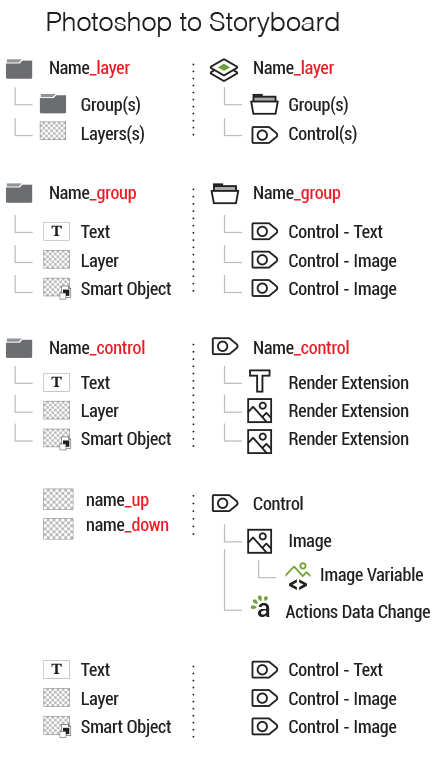
\includegraphics[width=8cm]{img/3_entwicklung_neues_kontept/story_psd}
	\caption[Hierarchie Modell für den Import von Photoshop-Dateien in Storyboard]{Hierarchie Modell für den Import von Photoshop-Dateien in Storyboard \cite{storyboard_doku_psd}}
	\label{fig:story_psd}
\end{figure}

Die Grafiken werden in bestimmten Ebenen gruppiert und nach einem Schema benannt. In Abbildung \ref{fig:story_psd} ist die Hierarchie zu sehen. Auf der linken Seite sind die Photoshop relevanten Elemente abgebildet, rechts daneben die Storyboard betreffenden.\\

Ein Ordner der in Photoshop mit \glqq \_layer\grqq{} endet wird auch als Layer in Storyboard eingefügt. Unterhalb dieses Layers, kann eine weitere Gruppierung existieren, sowie eine oder mehrere Photoshop-Ebenen.\\

Die Endung \glqq \_group\grqq{} erstellt eine Gruppierung in Storyboard. Innerhalb der Gruppe können sich Ebenen, Textebenen, sowie Smart Objects befinden. Jede dieser Ebenen wird zu einem Control in Storyboard. Ein Control Objekt besteht in Storyboard aus Render Extensions. Render Extension können Text, Bilder, Kreisbögen und ähnliches sein.\\

Gruppierungen mit der Endung \glqq \_control\grqq{} fassen ein Control Objekt in Storyboard zusammen. Alle Ebenen darunter werden zu Render Extensions die zu dem Control Objekt gehören. Mit Render Extensions können Control Objects einfache bis komplexe Aufgaben erfüllen. Ein Control Object mit zwei Image Render Extensions kann z.B. einen Button im Normal- und Gedrückt-Zustand darstellen.\\

Ein Button kann ebenfalls aus Photoshop importiert werden. Dazu wird ein Photoshop-Layer mit \glqq name\_up\grqq{} und \glqq name\_down\grqq{} benötigt. Storyboard erstellt aus diesen zwei Layern, ein Control Object mit einer Image Render Extension. Das Ändern des Bildes wird hier mit einer \glqq Image Variable\grqq{} und einer Action realisiert. Die Action wird aktiviert sobald innerhalb des Buttons geklickt wird und ändert dann die Quelle für das Bild in der \glqq Image Variable\grqq{}. Einzelne Layer, mit oder ohne Text, werden in Control Objects mit entsprechender Render Extension umgewandelt.\\


Für den Import in Storyboard wurde eine Photoshop-Datei erstellt. Die Photoshop-Datei besteht aus zwei Nadelinstrumenten, wie es von den Use Cases aus den vorherigen Kapiteln gefordert ist. Jedes Nadelinstrument besteht aus einem Hintergrund, dem äußeren Kreisbogen mit Zahlen, der Nadel, dem inneren Ring und der digitalen Anzeige. In der Datei gibt es zusätzlich noch zwei ausgeblendete Layer \glqq Overlay\_Layer\grqq{} und \glqq Telltales\_Group\grqq{}. Damit bei einem Import nicht direkt alle Layer in den aktiven Bildschirm geladen werden, können verschieden Layer ausgeblendet werden. Ausgeblendete Layer werden als \glqq Unused Layer\grqq{} importiert und können später bei Bedarf eingefügt werden.\\

\begin{figure}[htb]
	\centering
	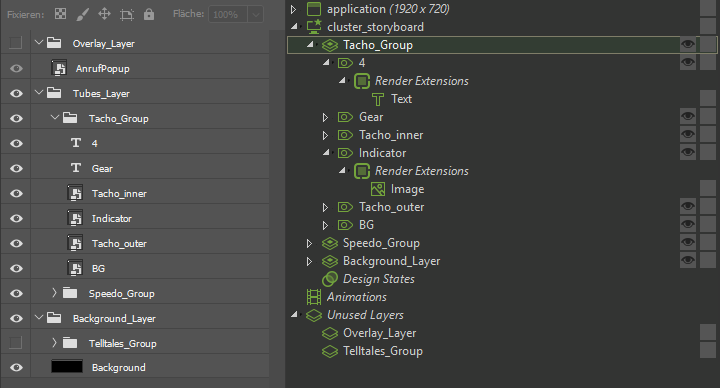
\includegraphics[width=\textwidth]{img/3_entwicklung_neues_kontept/vgl_psd_story}
	\caption[Vergleich Photoshop-Ebenen mit Storyboard-Ebenen]{Vergleich Photoshop-Ebenen (links) mit Storyboard-Ebenen (rechts)}
	\label{fig:vgl_layer}
\end{figure}

\newpage

In Abbildung \ref{fig:vgl_layer} ist die Aufteilung der Ebenen zu sehen. Links ist die Aufteilung in Photoshop zu sehen, rechts die Aufteilung in Storyboard direkt nach dem Import. In Photoshop wurden zwei Gruppen-Ordner angelegt unterhalb des \glqq Tube\_Layer\grqq{}. Zum einen die \glqq Tacho\_Group\grqq{} und zum anderen die \glqq Speed\_Group\grqq{}. Diese beiden Gruppen werden ebenfalls als Gruppierung in Storyboard eingefügt. Als Beispiel wird die \glqq Tacho\_Group\grqq{} genommen. Unterhalb der Gruppe in Photoshop, sind zwei Text-Ebenen und vier Ebenen mit Grafiken. In Storyboard werden diese Ebenen als Control mit den entsprechenden Render Extension eingefügt. Die Ebene \glqq 4\grqq{} ist in Photoshop eine Text-Ebene und wird in Storyboard als Control mit einer Text Render Extension eingefügt. Das selbe gilt für die Grafiken z.B. in Layer \glqq Tacho\_inner\grqq{} ist in Photoshop eine Ebene mit Grafik, in Storyboard wird hierfür ein Control mit einer Image Render Extension erstellt.

\subsubsection{Cluster HMI}

Der erste Use Case beschäftigt sich vor allem mit Nadelinstrumenten. In diesem Unterkapitel wird darauf eingegangen wie ein Nadelinstrument in Storyboard umgesetzt wird.\\

Ausgangspunkt ist ein Projekt direkt nach dem Import der Photoshop-Datei aus dem vorherigen Kapitel. Die zwei Nadelinstrumente aus der Photoshop-Datei werden korrekt in der Szene dargestellt. Zunächst muss die Größe des Controls mit der Nadelgrafik angepasst werden. Die Größe muss dem äußeren Ring aus Abbildung \ref{fig:img_prop_outer_tacho} entsprechen. Der äußere Ring ist ein Kreisbogen. Das Control-Element besitzt eine Breite von 548 Pixeln, was dem Durchmesser entspricht. Aufgrund der Abschrägung auf der Unterseite ergibt sich eine Höhe von 495 Pixeln. Das Control Object der Nadel muss die selbe Größe haben damit sich der Rotationspunkt an der richtigen Position befindet.\\

\begin{figure}[htb]
	\centering
	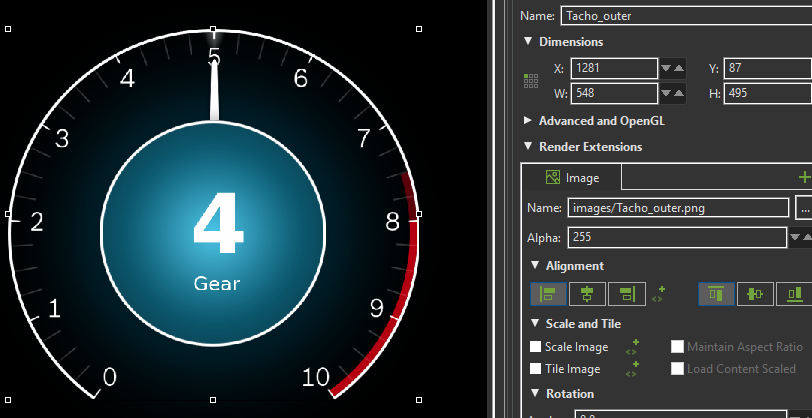
\includegraphics[width=\textwidth]{img/4_hmi_tools/anpassung_indicator}
	\caption{Grafik und Eigenschaften des äußeren Rings des Tachos}
	\label{fig:img_prop_outer_tacho}
\end{figure}

Innerhalb des Control-Elements muss die Grafik um 261 Pixel nach rechts verschoben werden, da die Grafik eine Breite von 26 Pixeln besitzt. Ansonsten würde die Nadel in der oberen linken Ecke dargestellt werden und nicht mittig. Anschließend müssen nur noch die Einstellungen für die Rotation vorgenommen werden. Das Rotationszentrum muss auf die Mitte des Control-Elements gelegt werden. \glqq Rotate around center of control\grqq{} führt nicht zum gewünschten Ergebnis. Für eine korrekte Rotation muss der X- und Y-Wert jeweils auf 274 gesetzt werden, die Hälfte von 548. Wird der Winkel jetzt verändert, rotiert die Nadel direkt am äußeren Ring entlang.\\

Damit während der Simulation die Nadel bewegt werden kann, muss mit Events und LUA-Skripten gearbeitet werden. Mit den LUA-Skripten können komplexe Funktionen umgesetzt werden. LUA kann auf alle Eigenschaften der Render Extensions zugreifen und sie ändern.\\

Zunächst muss ein Event erstellt werden. Events können bei verschiedenen Ereignissen ausgelöst werden um benutzerdefinierte Funktionen ( z.B. in LUA) auszuführen. Das Event \glqq cluster\_update\grqq{} ermöglicht, dass während der Simulation verschiedene Werte veränderbar sind.\\

\begin{figure}[htb]
	\centering
	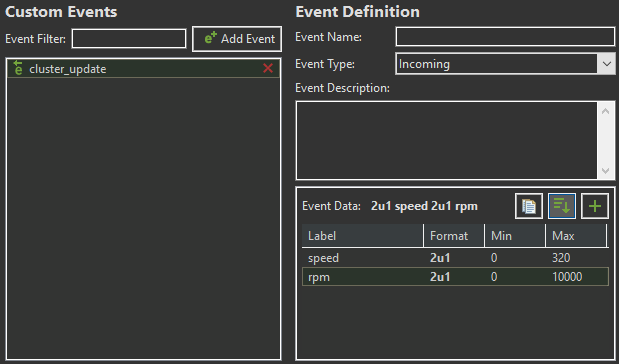
\includegraphics[width=\textwidth]{img/4_hmi_tools/event_indi_story}
	\caption{Cluster Update in Event Storyboard}
	\label{fig:event_story}
\end{figure}

Jeder Wert der änderbar sein soll, muss im Event als Label angelegt werden. Ein Label besteht aus einem Namen, Datentyp, minimalem Wert und maximalem Wert. In Abbildung \ref{fig:event_story} ist ein beispielhaftes Event mit Labeln abgebildet. Das Event ist über den Storyboard Connector erreichbar. Dort kann das Event ausgewählt und die Werte können über Schieberegler verändert werden.\\

In der callbacks.lua wird eine Funktion erstellt, welche ebenfalls \glqq cluster\_update\grqq{} heißt. Um eine bessere Übersichtlichkeit zu gewährleisten werden das Event und die dazugehörige Funktion gleich benannt. Die callbacks.lua ist die Hauptskript-Datei, in der alle Funktionen implementiert werden die nötig sind. \\

\newpage

\lstset{language=[5.0]Lua}
\begin{lstlisting}[frame=htrbl, caption={callbacks.lua}, label={lst:callbacks_story}]
function cluster_update(mapargs)
--get all label values 
local speed = mapargs.context_event_data.speed
local rpm = mapargs.context_event_data.rpm
local speed_rot = interpolation(speed,0,320,-144,144)
local rpm_rot = interpolation(rpm,0,10000,-144,144)

--set all variables
gre.set_value("Speedo_Group.speedo_indicator.rotation", speed_rot)
gre.set_value("Tacho_Group.Indicator.rotation", rpm_rot)
end

function interpolation(x,x1,x2,y1,y2)
return y1+(y2-y1)/(x2-x1)*(x-x1)
end
\end{lstlisting}

Die \glqq cluster\_update\grqq{} Funktion, in Listing \ref{lst:callbacks_story}, muss alle Änderungen an den Werten einlesen und verarbeiten. Für das Nadelinstrument muss die Geschwindigkeit eingelesen und in einen Winkel umgerechnet werden. Mit \glqq mapargs.context\_event\_data.speed\grqq{} bzw. \glqq mapargs.context\_event\_data.rpm\grqq{} kann auf die Werte der Labels aus dem cluster\_update zugegriffen werden. Eine selbstgeschriebene Interpolationsfunktion berechnet aus der Geschwindigkeit einen Winkel für die Nadel. Anschließend wird mit der Funktion \glqq gre.set\_value()\grqq{} der berechnete Winkel an eine Variable ausgegeben.\\

Mit Hilfe einer Variablen können Eigenschaftswerte eines Control Objects zur Laufzeit verändert werden. Eine Variable kann über einen Rechtsklick auf ein Control Object erstellt werden. In dem sich öffnenden Fenster kann der Datentyp und der Name der Variable gewählt werden. Für die Nadelrotation wird eine Float Variable mit dem Namen \textit{rotation} erstellt. Im Eigenschaftsfenster des Control Objects muss die Variable mittels Databinding an die Eigenschaft \textit{Angle} gebunden werden. Das führt dazu, dass der Wert der Variable automatisch an die Eigenschaft weitergegeben wird.\\

Zum Schluss muss noch eine Action erstellt werden. Eine Action verbindet ein Event mit bestimmten Funktionen. In diesem Fall soll die LUA-Funktion \glqq cluster\_update\grqq{} ausgeführt werden, wenn das dazugehörige \glqq cluster\_update\grqq{} Event ausgelöst wird.\\

In der Mitte des linken Nadelinstruments muss die Geschwindigkeit zusätzlich digital angezeigt werden. Dazu muss zunächst ein Control Object mit einer Text Render Extension angelegt und korrekt positioniert werden. Mit der Text Render Extension lässt sich beliebiger Text anzeigen.\\

Das Control Object benötigt wieder eine Variable, dieses mal vom Datentyp String. Analog zur Nadelrotation, muss der Wert nun wieder in der \glqq cluster\_update\grqq{} Funktion eingelesen und in die Variable geschrieben werden. Über Databinding wird der Wert der Variable an die Eigenschaft \textit{Text} weitergegeben.\\

%bis hierhin neu

Unterhalb der digitalen Geschwindigkeit muss die dazugehörige Einheit angezeigt werden. Zusätzlich soll die Einheit umschaltbar zwischen Meilen und Kilometern pro Stunde sein.\\

Dem Control Object der digitalen Geschwindigkeit wird dazu eine weitere Text Render Extension hinzugefügt. Wie auch bei der Geschwindigkeitsanzeige muss auch hier eine Variable erstellt und die Verarbeitung in LUA programmiert werden. Allerdings muss dieses mal ein neues Label im \glqq cluster\_update\grqq{} Event angelegt werden. Für ein Umschalten zwischen zwei Zuständen, ist eine boolesche Variable ausreichend.\\

Als letztes wird noch ein Nachleuchten-Effekt benötigt. Der Nachleuchten-Effekt soll die Bewegung der Nadel verdeutlichen. Die für diesen Effekt erstellte Grafik, reicht von 0 bis 160 \si[per-mode=symbol]{\kilo\meter\per\hour} und nimmt damit genau die Hälfte des Nadelinstruments ein. Da sich die Geschwindigkeit stetig verändert, bewegt sich auch die Nadel. Bewegt sich die Nadel im Bereich unterhalb der 160 \si[per-mode=symbol]{\kilo\meter\per\hour} muss ein Teil der Grafik ausgeblendet werden. Also der Teil der von der Nadel bis zu 160 \si[per-mode=symbol]{\kilo\meter\per\hour} reicht. Bewegt sich die Nadel allerdings im Bereich oberhalb der 160 \si[per-mode=symbol]{\kilo\meter\per\hour} muss die komplette Grafik mit der Nadel rotieren.\\

Eine Maske wäre für diesen Effekt die beste Lösung. Durch eine Maskierung der Grafik, kann der nicht benötigte Teil ausgeblendet werden. Die Maske würde in diesem Fall aus einem Kreisbogen bestehen, der immer vom Anfang des Nadelinstruments bis zur Nadel reicht. Das Ende des Kreisbogens folgt also dynamisch der Nadel. Die Pixel der Grafik würden dann nur angezeigt werden wenn an dieser Stelle, auch ein Pixel in der Maske gesetzt ist.\\

Storyboard bietet allerdings keine Möglichkeit Masken zu benutzen. Auf Nachfrage beim Support wurde eine Lösung genannt die auf Shadern basiert. Die Anzahl an Shadern in eingebetteten System ist allerdings begrenzt. Das heißt, Shader sollten sparsam verwendet werden. Da es wichtigere Funktionen gibt als den Nachleuchten-Effekt, die zwingend Shader verwenden müssen, ist diese Lösung nicht nutzbar.\\

Zusammenfassend lässt sich sagen, dass sich die Use Cases aus diesem Kapitel leicht umsetzen lassen. Der Photoshop Import erleichtert das Einfügen von Elementen, da sie im voraus bereits in Photoshop platziert werden können. Somit lässt sich z.B. das Nadelinstrument innerhalb von wenigen Minuten einfügen. Allerdings ist die Erstellung der Funkionen in LUA außerordentlich aufwendig. Zudem ist es nicht möglich einen Nachleuchten-Effekt mittels Maskierung zu erstellen. Das führt dazu das Storyboard in der späteren Auswahl nicht berücksichtigt werden kann.\\

\subsubsection{Visual Appearance}
In diesem Kapitel geht es um die Darstellung der \ac{ACC}-Funktion. Der Zustand der \ac{ACC}-Funktion muss mit einem 3D-Modell eines Fahrzeugs dargestellt werden.\\

Ein 3D-Modell wird in Storyboard mit Hilfe der 3D-Model Render Extension umgesetzt. Sobald ein Control Object mit einer 3D Render Extension erstellt wird, öffnet sich ein Datei-Dialog (Abbildung \ref{fig:story_import}). In diesem Dialog kann ein bereits importiertes 3D-Modell ausgewählt oder eine neues importiert werden.\\

\begin{figure}[htb]
	\centering
	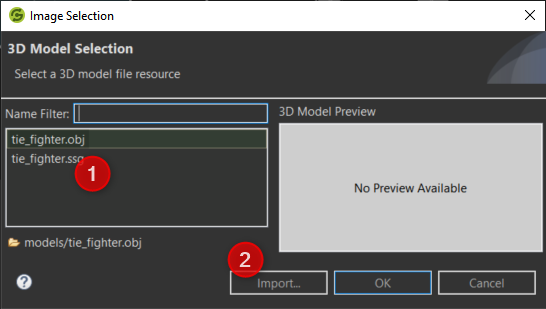
\includegraphics[width=12cm]{img/4_hmi_tools/model_import_story}
	\caption[3D-Modell Import Dialog in Storyboard]{3D-Modell Import Dialog 1:importierte Modelle, 2:Import Button für neue Modelle}
	\label{fig:story_import}
\end{figure}


Eine 3D-Szene besteht aus einem 3D-Objekt, einer Kamera und einem Licht. Die Kamera ist in dem Fall immer die Szene auf der gerendert wird. Das Licht sorgt dafür, dass realistische Schatten auf das 3D-Objekt fallen. Die 3D-Modell Render Extension besitzt eine größere Menge von Einstellungen, die in Abbildung \ref{fig:3d_model_story} dargestellt sind. Im Folgenden wird nur auf die wichtigsten Eigenschaften eingegangen.\\

\begin{figure}[htb]
	\centering
	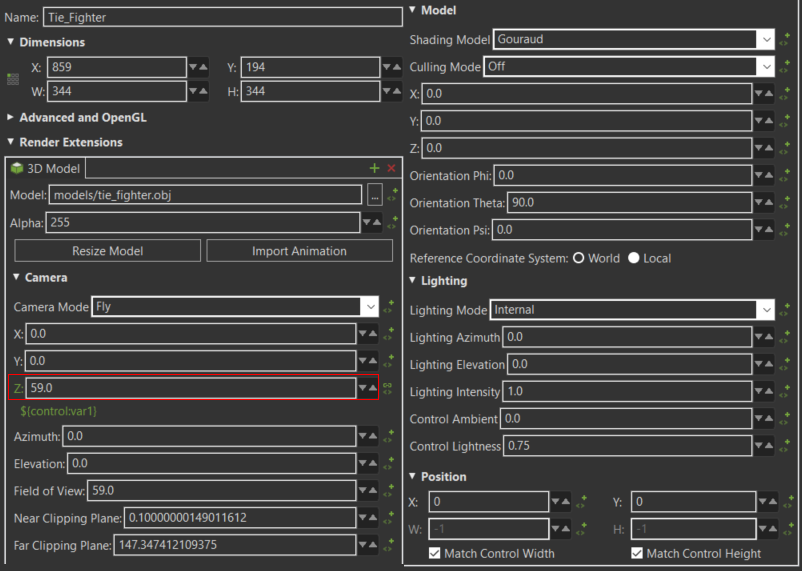
\includegraphics[width=\textwidth]{img/4_hmi_tools/3d_model_props}
	\caption[Einstellungen eines 3D-Models in Storyboard]{Einstellungen eines 3D-Models}
	\label{fig:3d_model_story}
\end{figure}

\newpage

Das 3D-Modell muss sich abhängig von der Geschwindigkeit nach vorne oder nach hinten bewegen. Diese Anforderung lässt sich in drei verschiedenen Varianten umsetzten. Zum einen kann die Eigenschaft Field of View verändert werden. Diese Eigenschaft verändert das Sichtfeld der Kamera. Ein höhere Wert sorgt dafür, dass das Modell kleiner wird. Ein kleinerer Wert lässt das Modell größer werden. Zum anderen kann die Kamera oder das Objekt über die Koordinaten bewegt werden.\\

Für die Umsetzung des Use Cases wird die Kamera in Z-Richtung bewegt. Die restliche Vorgehensweise ist analog zu den vorherigen Beispielen. Es wird wieder eine Variable benötigt und in LUA muss eine Verarbeitung der Werte stattfinden.

\subsubsection{Text- und Listenverhalten}
Im Use Case Text- und Listenverhalten muss eine scrollbare Liste umgesetzt werden. Die Liste sollte ca. 500 Einträge enthalten.\\

Um eine Liste in Storyboard zu erstellen, wird eine Tabelle benötigt. Zur Laufzeit kann diese Tabelle dynamisch mit Daten gefüllt werden. Zunächst muss eine Tabelle mit einer Spalte und einer Zeile erstellt werden. Die Tabelle wird später in LUA an die Anzahl der Einträge angepasst. Damit die Einträge dynamisch verändert werden können, wird eine Tabellen Variable benötigt. In diese Variable wird der Inhalt geschrieben, über Databinding werden die Daten an die Tabelle weitergegeben.\\

\lstset{language=[5.0]Lua}
\begin{lstlisting}[frame=htrbl, caption={callbacks.lua}, label={lst:callbacks_story}]
function CBInitTable()

-- read data
local file = assert(loadfile(gre.SCRIPT_ROOT .. "/words/wordList.txt"))
local words = file()

-- set table to 500 entries
gre.set_table_attrs("ListBehaviour.Playlist", {rows = 500})

-- save data in temp var
local data = {}
for row=1,500 do
data[string.format("ListBehaviour.Playlist.name.%d.1", row)] = words[row]

end

-- write data to variable
gre.set_data(data)
end
\end{lstlisting}

Als Quelle dient eine Textdatei, in dieser Datei sind alle Einträge enthalten. Damit die Liste zum Programmstart gefüllt wird, muss die Funktion aus Listing \ref{lst:callbacks_story} über eine Action ausgeführt werden. Die Funktion \textit{CBInitTable} liest die Einträge aus der \textit{wordList.txt} aus und schreibt sie in die Tabellen Variable.\\

In den Eigenschaften der Tabelle lässt sich noch einstellen wie gescrollt wird. Zur Auswahl steht einmal, von Eintrag zu Eintrag, oder pixelbasiert.\\

\subsubsection{Externe Daten}
Im Use Case Externe Daten soll überprüft werden, ob es möglich ist ein Video aus externer Quelle abzuspielen (z.B. Navigationsbild, Rückfahrkamera). \\

Damit ein Video in Storyboard abgespielt werden kann, wird ein Control Object mit der External Buffer Render Extension benötigt. In diesem Buffer können verschiedene externe Inhalte gerendert werden (z.B. Webbrowser oder Videos).\\

Um den Buffer mit einem Video zu befüllen, muss die Funktion \textit{gra.media.new.video} ausgeführt werden. Die Funktion wird von Storyboard bereitgestellt und wird nur über die Eigenschaften im Eigenschaftsfenster spezifiziert. In den Eigenschaften wird der Channel Name, die Video Quelle, sowie der External Buffer festgelegt. Der Channel Name ist wichtig, falls mit einer anderen Funktion das Video z.B. pausiert werden soll. In beiden Funktionen muss dann der gleiche Name stehen. Die Eigenschaft External Buffer Name stellt die Verbindung zum vorher erstellten External Buffer her.\\

Damit die Funktion \textit{gra.media.new.video} ausgeführt wird, wird ein Event benötigt. Dazu wird das Event \textit{MediaPlay} angelegt. Das Event kann z.B. über einen Klick auf einen Button ausgelöst werden und das Video wird abgespielt. Damit das Video gestoppt werden kann, wird noch das Event \textit{MediaStop} angelegt. Dieses Event löst die Funktion \textit{gra.media.stop} aus.\\

In diesem Fall soll das Video über den Storyboard Connector gestartet und gestoppt werden. Im \textit{cluster\_update} Event wird dazu ein neues Label erstellt. Das Label ist eine boolesche Variable. Mit diesen zwei Zuständen werden die zwei Events, \textit{MediaPlay} und \textit{MediaStop} ausgelöst. Bei dem booleschen Wert false wird das Video gestoppt und bei true wird das Video abgespielt.\\

Das Auslösen der Events erfolgt in der \textit{cluster\_update} Funktion. In Listing \ref{lst:media_story} ist der Code zu sehen. Zunächst wird der aktuelle Wert des Labels ausgelesen, anschließend wird je nach Zustand ein Event ausgelöst.\\

\begin{lstlisting}[frame=htrbl, caption={callbacks.lua}, label={lst:media_story}]
local play = mapargs.context_event_data.playVideo
if play == 1 then
	gre.send_event("MediaPlay")
	playerAttr["hidden"] = 0
	gre.set_control_attrs("VideoPlayback",playerAttr)
else
	gre.send_event("MediaStop")
	playerAttr["hidden"] = 1
	gre.set_control_attrs("VideoPlayback",playerAttr)
end
\end{lstlisting}

Abschließend lässt sich sagen, dass sich mit Storyboard der Großteil der Use Cases umsetzen lässt. Einzig der Nachleuchten-Effekt ist nicht umsetzbar. Der grafische Teil der Use Cases ist meist schnell realisiert, allerdings ist das Erstellen der einzelnen Funktionen dahinter mühselig. Oft muss für eine einfache Funktion ein Event, eine Action und eine LUA-Funktion erstellt werden, auch für relativ triviale Funktionen. Das sorgt in größeren Projekten für eine schlechte Übersichtlichkeit, zudem erschwert das die Modifizierbarkeit. Muss eine Funktion geändert werden, muss eventuell das Event, die Action und die LUA-Funktion verändert werden. Qt bietet dazu mit dem Qt Design Studio einen Kontrast und wird deshalb im nächsten Kapitel evaluiert.\\

\subsection{Qt}
\label{qt}
Qt wurde das erste mal 1995 von der Firma Trolltech veröffentlicht. Qt war damals noch ein Framework und keine komplette Entwicklungsumgebung. Entwickelt wurde dieses Framework von zwei norwegischen Entwickeln, Haavard Nord und Eirik Chambe-Eng. Heute besteht Qt aus einer umfangreichen Entwicklungsumgebung, dem QtCreator, sowie einem Design Tool, dem Qt Design Studio. \cite{qt_company}\\

Im Qt Design Studio werden die einzelnen grafischen Elemente zu einem \ac{HMI} zusammengefügt. Qt hat dafür eine eigene Skriptsprache entwickelt. \ac{QML} ist angelehnt an CSS und JSON und gehört zu den Auszeichnungssprachen (engl. Markup Language). Auszeichnungssprachen sind für die Gliederung und Formatierung von Text, Daten, etc. gedacht. Innerhalb von \ac{QML} kann zusätzlich die Javascript Syntax verwendet werden.\\

\subsubsection{Photoshop Import}

Als Verbindung zwischen Photoshop und Qt bietet Qt ein Plugin für Photoshop an. Die Photoshop Bridge wird als zxp-Datei geliefert und lässt sich über den ZXP Installer installieren. Das Photoshop Plugin wurde im Rahmen der Arbeit nicht evaluiert, daher wird nicht näher darauf eingegangen.\\


\subsubsection{Cluster HMI}
In diesem Use Case muss wieder ein Nadelinstrument umgesetzt werden.\\

Das Nadelinstrument wird mit der Image-Komponente zusammengestellt. Für jede Grafik des Nadelinstruments wird eine Image-Komponente im Qt Design Studio erstellt. Die Komponenten müssen in der Hierarchie anschließend in die richtige Reihenfolge gebracht werden, damit das Nadelinstrument korrekt dargestellt wird. Im Qt Design Studio steht die unterste Ebene in der Hierarchie an erster Stelle.\\

Um die Rotation der Nadel zu ermöglichen, wird die Item-Komponente benötigt. Ein Item kann als Container verstanden werden. In einem Item können sich mehrere Objekte befinden. Diese Objekte können dann z.B. im Koordinatensystem des Items positioniert werden. Im Fall der Nadel kann die Grafik an einer bestimmten Position um einen bestimmten Punkt rotieren. Das heißt Die Nadel wird im Koordinatensystem der Item-Komponente Positioniert und die Item-Komponente wird mittig im Nadelinstrument positioniert. Anschließend kann über die Eigenschaft \textit{rotation} die Nadel rotiert werden.\\

%nadelrotation fertig

In der Mitte des Nadelinstruments muss die Geschwindigkeit wieder digital angezeigt werden. Außerdem wird auch wieder die umschaltbare Einheit benötigt. Beide Funktionen sind mit der Text-Komponente umsetzbar. Über die Eigenschaft \textit{text} kann der angezeigte Text jederzeit verändert werden.\\

%digital fertig

Die Nadel soll einen Nachleuchten-Effekt besitzen. Qt bietet dafür die OpacityMask-Komponenten. Mit dieser Komponente lassen sich Grafiken einfach maskieren. In Abbildung \ref{fig:qt_mask} ist eine Übersicht zur Maske dargestellt.\\

\begin{figure}[htb]
	\centering
	
\includegraphics[width=\textwidth]{img/4_hmi_tools/qt_mask}
	\caption[Maskierung einer Grafik in Qt]{Maskierung einer Grafik. Links das Ursprungsbild, in der Mitte die Maskengrafik, rechts das maskierte Ursprungsbild. \cite{qt_mask}}
	\label{fig:qt_mask}
\end{figure} 

Die Maske besteht aus einem Ursprungsbild und der Maskengrafik. Ein Pixel im Ursprungsbild wird nur angezeigt, wenn in der Maskengrafik an der gleichen Position auch ein Pixel ist. Ist der Pixel an der gleichen Position nicht vorhanden, wird der Pixel des Ursprungsbildes ausgeblendet.\\

Mit dieser Komponente lässt sich der Nachleuchten-Effekt umsetzten. Das Ursprungsbild ist die Nachleuchten-Grafik und die Maskengrafik ist ein Kreisbogen (Arc). Der Kreisbogen wird mit der Arc-Komponente umgesetzt. Der Arc startet bei 0 \si[per-mode=symbol]{\kilo\meter\per\hour} und endet immer an der Nadel. Dadurch wird die Nachleuchten Grafik immer nur dort angezeigt, wo sie benötigt wird. Das mit rotieren der Grafik ab 160 \si[per-mode=symbol]{\kilo\meter\per\hour} ist entweder über eine Animation oder über eine Simulation mit Javascript umsetzbar.\\

Um die Bewegung der Nadel und den Nachleuchten-Effekt mit einer Animation zu lösen, wird zunächst eine neue Animation-Timeline erstellt. In der Animation-Timeline können für die verschiedenen Komponenten Keyframes festgelegt werden. Eine Animation besteht aus mehreren Frames. Ein Keyframe legt den Wert einer Eigenschaft in einem bestimmten Frame fest. Zwischen zwei Werten in unterschiedlichen Frames wird interpoliert. Für die Nadel wird im ersten Frame die Eigenschaft \textit{rotation} so festgelegt, dass 0 \si[per-mode=symbol]{\kilo\meter\per\hour} angezeigt werden. Anschließend wird ein Keyframe erstellt und die Rotation in der Timeline gespeichert. Danach muss die Nadel auf die Endposition, damit im letzten Frame erneut die Rotation mit einem Keyframe gespeichert werden kann. Beim Abspielen der Timeline bewegt sich die Nadel nun von 0 bis 320 \si[per-mode=symbol]{\kilo\meter\per\hour}. Das gleiche muss für die anderen Komponenten vorgenommen werden, damit auch der Nachleuchten-Effekt korrekt dargestellt wird.\\

Die Animation besteht insgesamt aus 320 Frames. Jeder Frame stellt damit genau 1 \si[per-mode=symbol]{\kilo\meter\per\hour} dar. Somit benötigt die QML-Datei später nur die Geschwindigkeit, da die Geschwindigkeit mit einem Frame der Animation gleichzusetzen ist. Zudem müssen keine Berechnungen in QML stattfinden.\\

%gefällt mir noch nicht
Für die Simulation im Qt Design Studio besteht die Möglichkeit mit Javascript ein Backend zu erstellen. Hierzu wird eine Javascript-Datei und eine QML-Datei erstellt. In der QML-Datei werden die benötigten Variablen und Timer programmiert. Ein Timer ruft in einem bestimmten Intervall eine Funktion aus der Javascript-Datei auf. In der Javascript Funktion wird dann ein Wert hoch- oder runtergezählt, z.B. die Geschwindigkeit. Der Wert wird in der QML zwischengespeichert und kann in einer anderen QML über Databinding an eine Eigenschaft übergeben werden.\\

%noch mehr dazu?
Der Use Case Cluster HMI erfordert ebenfalls die Implementierung von Warnlampen. Qt bietet dafür eine eigene Komponente, die IsoIcon-Komponente. IsoIcons können beliebig platziert werden. Ein Doppelklick auf das Element öffnet einen Auswahl-Dialog. In diesem Dialog sind alle Icons nach dem ISO Standard auswählbar. Über die Eigenschaften kann anschließend die Farbe konfiguriert werden.\\

\subsubsection{Visual Appearence}
Dieses Kapitel beschäftigt sich mit dem Anzeigen der \ac{ACC}-Funktion. Hierzu muss wieder ein 3D-Modell darstellbar sein. Qt bietet für 3D-Szenen QtQuick3D an. \\

Um 3D Modelle im FBX Format in QML zu nutzen, bietet Qt eine Import-Funktion an. Mit Hilfe der Import-Funktion wird aus dem 3D-Modell eine eigene QML-Datei erzeugt. Die QML-Datei wird später als benutzerdefinierte QML-Komponente benutzbar und kann dadurch in anderen QML-Dateien verwendet werden.\\

Im Qt Design Studio gibt es einen integrierten 3D-Editor. Es kann zwischen dem normalen Form-Editor und dem 3D-Editor gewechselt werden. Im Form-Editor werden die 2D QML-Komponenten dargestellt und können dort auch positioniert werden. Im 3D-Editor können alle 3D-Objekte wie z.B. Lichter, Modelle und Kameras positioniert, rotiert und skaliert werden. Im Form-Editor wird immer das aktuelle Kamerabild gerendert dargestellt. Abbildung \ref{fig:qt_3d} zeigt den 3D-Editor des Qt Design Studios.\\ 

\begin{figure}[htb]
	\centering
	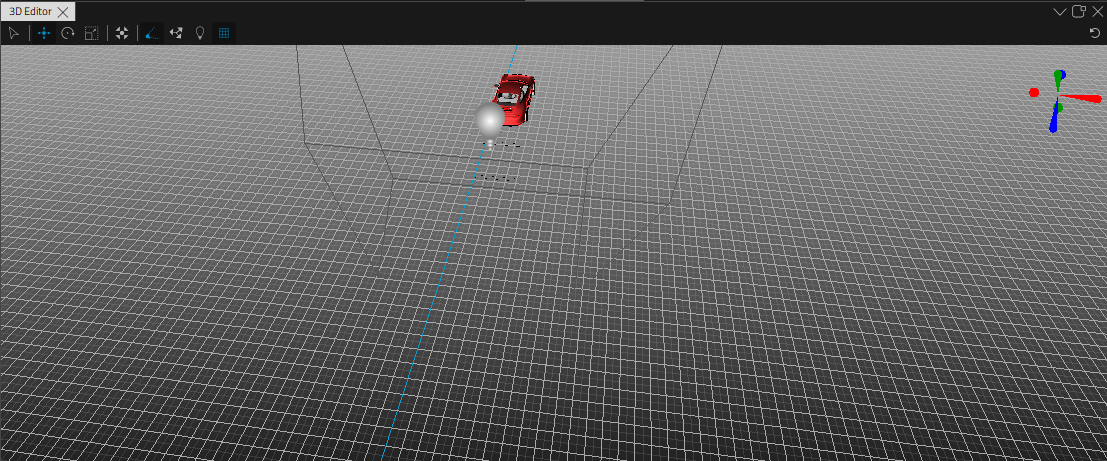
\includegraphics[width=\textwidth]{img/4_hmi_tools/3d_editor}
	\caption[3D-Editor in Qt]{Übersicht 3D-Editor im Qt Design Studio}
	\label{fig:qt_3d}
\end{figure}

Sobald alle Objekte in Position sind, muss noch die Y-Position des Autos als Alias exportiert werden. Ein Alias ermöglicht die Bearbeitung von internen Eigenschaften von außen. Die QML-Datei des 3D-Modells wird später in einer anderen QML-Datei verwendet. Ohne ein Alias wäre es nicht möglich auf die Y-Position des Fahrzeugs zuzugreifen. In der QML-Datei in der das 3D-Modell verwendet wird, lässt sich das Fahrzeug nach vorne oder hinten bewegen.\\

\begin{figure}[htb]
	\centering
	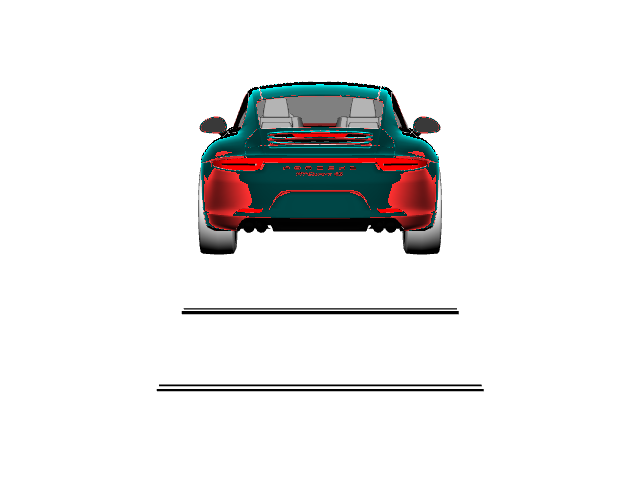
\includegraphics[width=\textwidth]{img/4_hmi_tools/qt_3d_render}
	\caption[Gerendertes Kamerabild einer 3D-Szene in Qt]{Das gerenderte Kamerabild als 3D-Szene in Qt}
	\label{fig:qt_render}
\end{figure}

Die fertige 3D-Szene ist in Abbildung \ref{fig:qt_render} zu sehen. Die Szene zeigt die Perspektive aus Sicht der Kamera. Die Szene ist im Form-Editor beliebig platzierbar.\\

\subsubsection{Text- und Listenverhalten}
%einleitender Satz

In Qt Design Studio werden Listen mit der Model/View Architektur erzeugt. Für die Liste wird dazu ein ListModel und eine ListView benötigt. Im ListModel werden die Daten hinterlegt und in der ListView angezeigt. Die Daten aus dem ListModel werden über ein Delegate an die ListView weitergegeben, ähnlich zum Beobachter-Muster. Diese vorgehensweise ist ähnlich zu dem \ac{MVC}-Muster.\\

%bild von https://doc.qt.io/qt-5/model-view-programming.html einfügen

Für die Evaluierung wird eine Liste mit dem XmlListModel erzeugt. Das XmlListModel bietet die Möglichkeit eine Liste in einer XML-Datei zu hinterlegen.\\

\newpage

\lstset{language=[5.0]Lua}
\begin{lstlisting}[frame=htrbl, caption={ListBehaviourModel.qml}, label={lst:list_qt}]
XmlListModel {
	id: xmlModel
	source: 																	"file:///C:/Users/plk4abt/Documents/instrumentCluster/backend/Data/listview_xml.xml"
	query: "/channel/item"

	XmlRole {
		name: "title"
		query: "title/string()"
	}
}
\end{lstlisting}

Listing \ref{lst:list_qt} veranschaulicht das Einbinden einer Xml-Datei. Die Daten sind damit im XmlListModel hinterlegt und können in einer ListView angezeigt werden. Die Daten aus dem XmlListModel werden über die Eigenschaft \textit{model} in die ListView geladen. Die Eigenschaft query in Zeile 4 gibt die Hierarchie in der XML-Datei vor. Das heißt jeder Listeneintrag muss zum einen innerhalb eines \textit{channel}-Tags liegen und zum anderen zwischen einem \textit{item}-Tag. In Zeile 7 wird festgelegt wo der Text für die Eigenschaft name hinterlegt ist. In diesem Fall liegt der Text zwischen dem \textit{title}-Tag. In Zeile 8 wird schließlich definiert, dass es sich um eine String-Variable handelt. Zum Vergleich ist in Listing \ref{lst:list_xml} ein Teil der XML-Datei abgebildet.\\

\lstset{language=[5.0]Lua}
\begin{lstlisting}[frame=htrbl, caption={list.xml}, label={lst:list_xml}]
<channel>
	<item>
		<title>A blog post</title>
	</item>
	<item>
		<title>Another blog post post</title>
	</item>
<\channel>
\end{lstlisting}


In der späteren Umsetzung wird auf ein eigenes Model zurückgegriffen. Dazu kann in C++ ein eigenes ListModel implementiert werden.\\ 

\subsubsection{Externe Daten}
Videos können im Qt Design Studio über die MediaPlayer-Komponente in die Video"=Output-Komponente geladen und abgespielt werden. In Listing \ref{lst:video_qt} ist der Code für den Videoplayer zu sehen.\\

\lstset{language=[5.0]Lua}
\begin{lstlisting}[frame=htrbl, caption={VideoPlayer.qml}, label={lst:video_qt}]
Item {
	width: Constants.width
	height: 720

	MediaPlayer {
		id: mediaplayer
		source: "file:///C:/Users/.../video/video.mp4"

	}

	VideoOutput {
		anchors.fill: parent
		source: mediaplayer

	}

	MouseArea {
		id: playArea
		anchors.fill: parent
		onPressed: mediaplayer.play();
	}
}
\end{lstlisting}

Die MediaPlayer-Komponente stellt die Quelldatei bereit, sowie Funktionen wie Play und Stop. Die Daten aus dem Video Player werden in den Buffer VideoOutput geladen, ähnlich wie in Storyboard. Die MouseArea-Komponente erlaubt das auslösen verschiedener Mausevents, z.B. einen Mausklick. Sobald innerhalb der MouseArea geklickt wird, wird mit \textit{mediaplayer.play()} das Video gestartet.\\

\subsection{Auswahl des HMI Tools}

Diese Kapitel beschäftigt sich mit der Auswahl des HMI Tools. Dafür werden alle Vor- und Nachteile aus den vorherigen Kapiteln gegenüber gestellt.\\

\subsubsection{Vor- und Nachteile CGI Studio}
CGI Studio wird schon mehrere Jahre bei Bosch verwendet. Durch die langjährige Nutzung, hat sich viel Fachwissen und Erfahrung im Umgang mit CGI Studio angesammelt. Bosch bestimmt zum Teil auch die Weiterentwicklung mit.\\

CGI Studio kann theoretisch alle benötigten Use Cases abdecken. Die Use Cases aus Kapitel \ref{use_cases} wurden aus CGI Studio abgeleitet. Doch wie in Kapitel \ref{cgi} beschrieben, gestaltete sich die praktische Umsetzung schwieriger als gedacht. Die Möglichkeit Widgets durch verschiedene DLL-Dateien zu laden, bietet Flexibilität, zeigt aber auch wie schnell das unübersichtlich wird. Vor dem Start, muss erst eine passende DLL-Datei gefunden werden und je mehr Projekte existieren, desto schwiergier wird die Suche.\\


\subsubsection{Vor- und Nachteile Storyboard}
Storyboard ist ein sehr einfach zu erlernendes Tool. Die Entwicklungsumgebung ist sehr übersichtlich. Da nur relativ wenige Render Extension zur Auswahl stehen, sind die Funktionen sehr begrenzt. Diese Begrenzung verringert aber gleichzeitig die Komplexität. Mit Hilfe von LUA lassen sich jedoch komplexere Funktionen umsetzen. Storyboard konnte nahezu alle Use Cases erfüllen. Die meisten Informationen sind in der ausführlichen Dokumentation zu finden, falls etwas nicht in der Dokumentation auffindbar ist, hilft der kommerzielle Support schnell weiter. \\

Bei manchen Use Cases gab es kleiner Probleme mit der Umsetzung. So ist das Erstellen von Übersetzungen unnötig kompliziert. Im Tool gibt es bereits eine Übersicht der Übersetzungen, jedoch können diese dort nicht bearbeitet werden. Stattdessen muss die CSV-Datei geöffnet und bearbeitet werden. Der größte Nachteil ist allerdings, dass der Nachleuchten Use Case nicht umgesetzt werden kann. Storyboard hat im Nachgang noch eine mögliche Lösung geliefert, allerdings basiert diese auf Shadern. Da die Anzahl der Shader begrenzt ist und für wichtigere Funktionen benötigt wird, ist diese Lösung nicht nutzbar. \\

Die Use Cases haben gezeigt, dass es möglich ist die View in Storyboard umzusetzen. Allerdings ist nicht ersichtlich wie der Rest der Architektur (Controller und Model) umzusetzen sind. Es existiert die Möglichkeit, Events als C bzw. C++ Header zu exportieren. Dadurch soll der Zugriff auf Events von außerhalb der Storyboard Anwendung möglich sein.\\
 %quelle http://resources.cranksoftware.com/cranksoftware/v6.0.0/docs/webhelp/ch07s03.html\\

\newpage
Damit wäre es theoretisch möglich die Architektur umzusetzen, allerdings müssten das Model und der Controller außerhalb von Storyboard implementiert werden.\\
 

\subsubsection{Vor- und Nachteile Qt}
%Qt besteht eigentlich nur aus dem Qt Creator. Innerhalb des Qt Creator gibt es noch das Design Studio und den Qt Designer. Beide Tools existieren ebenfalls als eigenständige Version. Wie im Kapitel \ref{qt} erläutert, wurden die Use Cases komplett im Design Studio umgesetzt. Die spätere Implementierung erfolgt allerdings im Qt Creator.\\

Ein großer Vorteil von Qt ist die Opensource Variante und die dadurch existierende Support Community. Durch die große Anzahl an Nutzern, werden Bugs schneller gefunden. In den vorhandenen Foren gibt es zudem eine Vielzahl von Fragen und Antworten rund um das Qt Framework. Kann eine Frage dadurch nicht beantwortet werden, bietet Qt noch einen kommerziellen Support. Das Qt-Framework beinhaltet von Haus aus sehr viele Funktionen, das spart Entwicklungsaufwand. Trotzdem können eigene Funktionen durch die Auszeichnungssprache QML entwickelt werden. Die Funktionen lassen sich später in jedem Projekt wiederverwenden, dadurch reduziert sich ebenfalls der Entwicklungsaufwand. Mit dem QtCreator stellt Qt zudem eine All-in-one Lösung bereit. Im QtCreator ist bereits das Qt Design Studio integriert. Dadurch können die Designer die \ac{HMI} im Qt Design Studio entwerfen und später die \ac{HMI} zum QtCreator Projekt hinzufügen.\\

Der große Funktionsumfang ist zeitgleich auch ein Nachteil. Vor allem am Anfang erschlägt Qt mit seiner Vielfalt. Das erhöht die Einarbeitungszeit im Vergleich zu Storyboard, liegt aber weiterhin deutlich unter der Einarbeitungszeit die für CGI Studio notwendig ist.\\

In Qt Design Studio lässt sich die View problemlos umsetzen. In Verbindung mit dem QtCreator, lassen sich ebenfalls das Model und der Controller implementieren.\\

\subsubsection{Auswahl des HMI Frameworks}

In Tabelle \ref{tab:tools} sind alle Vor- und Nachteile der einzelnen Frameworks zusammengefasst. Mit Hilfe dieser Übersicht muss ein \ac{HMI} Framework ausgewählt werden.\\

Storyboard kann bei der Auswahl nicht berücksichtigt werden, da ein must-have Use Case nicht erüllt werden kann. Die Auswahl muss also zwischen CGI Studio und Qt getroffen werden. Bei einem Vergleich der Vor- und Nachteile von Qt und CGI Studio gewinnt Qt. Während der Benutzung von Qt haben sich kaum Nachteile gezeigt. In Qt konnten alle wichtigen Use Cases zufriedenstellend umgesetzt werden. Nach einer kurzen Einarbeitungszeit funktioniert das Arbeiten in Qt flüssig. Auftretende Probleme konnten meist durch eine kurze Internetrecherche gelöst werden. Das Lösen der Probleme durch Internetrecherche ist der großen Community zu verdanken. Qt hat sehr viele Nutzer, dadurch werden auch viele Probleme gefunden und gelöst. Im Hinblick auf die ISO 25010 Kriterien, hilft das vor allem dem Punkt Reliability (Zuverlässigkeit). Dessen Unterpunkte in der Gewichtung zwischen 18 und 21 von 31 Punkten erreicht haben und damit zu den wichtigeren Punkten gehören.\\


Da die Use Cases von CGI Studio abgeleitet sind, kann CGI Studio alle Use Cases umsetzen. Die Probleme mit CGI Studio sorgen dafür, dass CGI Studio Qt unterliegt. Im Gegensatz zu Qt kann bei CGI Studio nicht im Internet recherchiert werden Es gibt einfach keine Nutzer außerhalb von Bosch, die im Internet nach Hilfe suchen. Bosch ist einer der Hauptnutzer und somit auch Tester von CGI Studio. Bugs und Fehler werden dadurch eventuell zu spät gefunden. Die Erfahrung hat gezeigt, dass es auch schwierig sein kann die richtige Person zu finden die, bei Problemen oder Fragen, helfen kann.\\



\begin{table}[h]
	\centering
	\caption[Übersicht der Vor- und Nachteile der einzelnen Frameworks]{Übersicht der Vor- und Nachteile der einzelnen Frameworks}
	\label{tab:tools}
	\begin{tabular}{|p{1.6cm}|p{4.3cm}|p{4.3cm}|p{4.3cm}|}
		\cline{2-4}
		\multicolumn{1}{c|}{}      & CGI Studio                                     & Storyboard                                  & Qt                                                  \\ \hline
		\multirow{15}{*}{Vorteile} & aktuelles Standard-Tool                        & schnelle Einarbeitung                       & All-in-one Lösung durch QtCreator                   \\ \cline{2-4}
		                           & viel Expertise innerhalb von Bosch             & ausführliche Dokumentation                  & ausführliche Dokumentation                          \\ \cline{2-4}
		                           & besitzt alle nötigen Funktionen                & simpler Photoshop Import                    & eigenes Photoshop Plugin                            \\ \cline{2-4}
		                           & Bosch bestimmt Weiterentwicklung mit           &                                             & große Anzahl an vorgefertigten Funktionen           \\ \cline{2-4}
		                           &                                                &                                             & Möglichkeit zur Entwicklung eigener Funktionen      \\ \cline{2-4}
		                           &                                                &                                             & Möglichkeit zur Wiederverwendung eigener Funktionen \\ \hline
		\multirow{9}{*}{Nachteile} & Kaum Support von außen möglich                 & hoher Implementierungsaufwand in LUA        & etwas längere Einarbeitungszeit nötig               \\ \cline{2-4}
		                           & Wissen konzentriert sich auf Projektbeteiligte & Übersetzungen hinzufügen kompliziert        &                                                     \\ \cline{2-4}
		                           & Veraltete Widgets sind fehleranfällig          & keine Masken-Funktion (Ausschlusskriterium) &                                                     \\ \hline
	\end{tabular} 
	
\end{table} 



Im Hinblick auf das Architektur-Konzept und die Vor- und Nachteile ist Qt die beste Wahl.\\


